%----------------------------------------------------------------------
\begin{frame}[c]{Where are we? The big picture}

\begin{itemize}
\item[$\to$] Algorithm Selection
  \begin{itemize}
    \item[$\to$] Portfolios
    \item Algorithm selection for runtime
  \end{itemize}
  \item Design Decisions:\\ Local Search + Evo. Algorithms + Machine Learning 
  \item Empirical evaluation
  \item AAD for ML
  \begin{itemize}
    \item Hyperparameter optimization and Bayesian Optimization 
    \item Neural architecture search (lecture given by Prof. Hutter)
  \end{itemize}
  \item Algorithm configuration 
  \begin{itemize}
    \item Basics 
    \item State of the art 
    \item Best Practices 
  \end{itemize}
  \item Combinations of algorithm selection and configurations
  \item Algorithm control 
  \item Algorithm analysis 
  \item Project announcment and questions for exam
\end{itemize}

\end{frame}
%----------------------------------------------------------------------
%----------------------------------------------------------------------
\begin{frame}[c]{}

\centering
\huge
Algorithm Portfolios and\\ Algorithm Selection

\bigskip
\includegraphics[width=0.8\textwidth]{images/algorithm_selection}

\end{frame}
%----------------------------------------------------------------------
%----------------------------------------------------------------------
\begin{frame}[c]{Motivation: Complementarity of Algorithms}

Real-world example (see SAT12-ALL scenario of ASlib):

\begin{itemize}
  \item Algorithm A (``sparrow'') on Instance X took $1.76$ sec
  \item Algorithm B (``glucose2'') on Instance X had a timeout ($\geq 1200$ sec)
  \pause
  \medskip
  \item Algorithm A (``sparrow'') on Instance Y had a timeout ($\geq 1200$ sec)
  \item Algorithm B (``glucose2'') on Instance Y took $24.1$ sec
\end{itemize}

\pause
$\leadsto$ Algorithms have different strengthes and weaknesses!

\pause
\bigskip
\begin{block}{Complementarity of Algorithms}
Two algorithms are complementary if they perform well on different kinds of instances.
\end{block}

\pause
(Definition of complementarity can be extended to sets of algorithms.)


\end{frame}
%-----------------------------------------------------------------------
%----------------------------------------------------------------------
\begin{frame}[c]{Learning Goals}

After this lecture, you will be able to \ldots

\begin{itemize}
  \item \alert{exploit complementarity} of algorithms to improve overall performance
  \item explain \alert{algorithm portfolios} and its different variants
  \begin{itemize}
    \item racing portfolios
    \item parallel portfolios
    \item algorithm schedules
  \end{itemize}
  \item define \alert{per-instance algorithm selection} and to describe one specific implementation 
  \item explain different types of \alert{instance features}
\end{itemize}

\end{frame}
%----------------------------------------------------------------------
%----------------------------------------------------------------------
\begin{frame}[c]{Prerequisite: Instances}

\begin{block}{What are instances?}
``Instances'' are inputs to an algorithm and the algorithm has to process instances.
In the end, the algorithm will return an output to an instance (a.k.a. the instance was ``solved'').
\end{block}

\pause

Synonyms:
\begin{itemize}
  \item Algorithm input
  \item Task
\end{itemize}

\pause

Examples:
\begin{itemize}
  \item Dataset for a machine learning algorithm
  \item Planning problem for an AI planning solver
  \item Mixed-integer program for a MIP solver
  \item CNF instance for a SAT solver
  \item Datatable for a database
\end{itemize}

\end{frame}
%----------------------------------------------------------------------
%----------------------------------------------------------------------
\begin{frame}[c]{Setting (today and next week)}

\includegraphics[width=0.9\textwidth]{images/as_setting}

\end{frame}
%----------------------------------------------------------------------

%----------------------------------------------------------------------
\begin{frame}[c]{Example: SAT Challenge 2012}

\centering
\includegraphics[scale=0.3]{images/satchallenge12_indu.png}

\begin{description}
  \item[green] A single algorithm on each instance
  \item[blue] A fixed set of algorithms solving each instance ``together''
  \item[pink] Algorithm selection approaches: Select the best algorithm for the instance at hand 
\end{description}

\end{frame}
%----------------------------------------------------------------------
%----------------------------------------------------------------------
\begin{frame}[c]{Oracle / Virtual Best Solver (VBS)}

\begin{block}{Intuition}
Given a portfolio (set) of algorithms, the oracle is the portfolio system
that always selects the best component algorithm for a given instance.
\end{block}

\pause
\bigskip

\begin{block}{Definition}
Given 
\begin{itemize}
  \item a portfolio (set) of algorithms $\portfolio$,
  \item a set of instances $\insts$,
  \item a cost metric $c: \portfolio \times \insts \to \perf$, 
\end{itemize} 
the cost of the oracle is $\sum_{\inst \in \insts} \min_{\algo \in \portfolio} c(\algo, \inst)$.
\end{block}

%Note: We do not consider information sharing between the algorithms in this setting.

\end{frame}
%-----------------------------------------------------------------------
%----------------------------------------------------------------------
\begin{frame}[c]{Toy Example: Oracle}

\[
\begin{array}{| r | c  c  c || c |}
  \cline{1-5}
      & \algo_1 & \algo_2 & \algo_3 & oracle\\
  \cline{1-5}
  \inst_1 & 		 1    &         10  &         3    & 1 \\
  \inst_2 &          5    &         10  &  		2 	  & 2 \\
  \inst_3 &          8    &  		1    &         10  & 1 \\
  \inst_4 &         10  &         10  & 		2 	  & 2 \\
  \inst_5 &         10  & 		 6    &         10  & 6 \\
  \inst_6 &         10  &          8    &         10  & 8 \\
  \cline{1-5}
  \onslide<2->{\varnothing & 7.3 & 7.5 & 6.1 & 3.3}\\
  %\text{timeouts} & 3 & 3 & 3 & 0 \\ 
  \cline{1-5}
\end{array}
\]


\end{frame}
%-----------------------------------------------------------------------
%----------------------------------------------------------------------
\begin{frame}[c]{Baseline: Single Best (SB)}

\begin{block}{Intuition}
If we don't use a portfolio, we would simply pick the best single algorithm.
\end{block}

\pause
\bigskip

\begin{block}{Definition}
Given a portfolio (set) of algorithms $\portfolio$, a set of instances $\insts$,
a cost metric $c: \portfolio \times \insts \to \perf$,
the single best (SB) algorithm is $\argmin_{\algo \in \portfolio} \sum_{\inst \in \insts} c(\algo, \inst)$
\end{block}

\pause
\bigskip

$\leadsto$ A portfolio system should have a performance\\ between the SB's performance and the oracle's performance.

\end{frame}
%-----------------------------------------------------------------------
%----------------------------------------------------------------------
\begin{frame}[c]{Toy Example: SB}

\[
\begin{array}{| r | c  c  c || c |}
  \cline{1-5}
      & \algo_1 & \algo_2 & \algo_3 & oracle\\
  \cline{1-5}
  \inst_1 & 		 1    &         10  &         3    & 1 \\
  \inst_2 &          5    &         10  &  		2 	  & 2 \\
  \inst_3 &          8    &  		1    &         10  & 1 \\
  \inst_4 &         10  &         10  & 		2 	  & 2 \\
  \inst_5 &         10  & 		 6    &         10  & 6 \\
  \inst_6 &         10  &          8    &         10  & 8 \\
  \cline{1-5}
  \varnothing & 7.3 & 7.5 & 6.1 & 3.3\\
  %\text{timeouts} & 3 & 3 & 3 & 0 \\ 
  \cline{1-5}
\end{array}
\]

\bigskip

$\to$ $\algo_3$ is the single best algorithm

\end{frame}
%-----------------------------------------------------------------------
\begin{frame}[c]{Oracle and SB in Practice}

\begin{tabular}{lrr}
\toprule
Domain 										& Oracle 	& Single Best \\
\midrule
Structure learning in Bayesian networks 	& $219.86$ 	& $9017.07$\\
Constraint Satisfaction Problem (CSP)		& $26.27$	& $1605.36$ \\
Maximum Satisfiability Problem (MAXSAT) 	& $101.34$	& $1572.00$\\
Mixed Integer Programming (MIP)				& $281.51$	& $3007.92$\\
Quantified Boolean Formula (QBF)			& $9.99$	& $2642.89$	\\
Boolean Satisfiability Problem 	(SAT12-ALL)	& $97.84$	& $2962.29$\\
\midrule
Machine Learning (OPENML-Weka; Error)		& $12.5\%$	& $14.5\%$\\
\bottomrule
\end{tabular}

\lit{Source: Open Algorithm Selection Challenge 2017}

\end{frame}
%----------------------------------------------------------------------
\begin{frame}[c]{Parallel algorithm portfolios~\litw{B. Huberman et al. 1997}}

\begin{block}{Definition}
Given a portfolio (set) of algorithms $\portfolio$ of size $k$ and $k$ parallel computation units (e.g., CPU cores),
a parallel portfolio system runs each $\algo \in \portfolio$ on one parallel computation unit in parallel.
The first $\algo$ that ``solved'' the instance at hand, terminates all other algorithms.  
\end{block}

\pause
$\leadsto$ Cost metric $c$ should relate to runtime of an algorithm. 


\bigskip
\pause

\begin{block}{Performance}
For a given set of instances $\insts$ and
a cost metric $c: \portfolio \times \insts \to \perf$,
the cost of a parallel algorithm portfolio is $\sum_{\inst \in \insts} \min_{\algo \in \portfolio} c(\algo, \inst) + \epsilon_{k}$
where $\epsilon_{k}$ is overhead induced by using $k$ parallel computation units in parallel.
\end{block}

\end{frame}
%-----------------------------------------------------------------------
%----------------------------------------------------------------------
\begin{frame}[c]{Parallel portfolios for SAT~\litw{Lindauer et al. 2017}}

\small
%\onslide<1->{PAR$X$ is the penalized average runtime where each timeout is counted as $X$ times the runtime cutoff.}

\begin{center}
\begin{tabular}{lrrrr}
\toprule
$\#$ Units   & \multicolumn{2}{c}{\lingeling} & \multicolumn{2}{c}{\clasp} \\
	 & \multicolumn{2}{c}{Industrial} & \multicolumn{2}{c}{Crafted}  \\
\midrule
& $\#$Timeouts & $\varnothing_t$ & $\#$Timeouts & $\varnothing_t$\\
\cmidrule{2-3}\cmidrule{4-5}
$1$ & $82$ & $380$ & $136$ & $464$\\
\pause
$2$ & $65$ & $331$ & $118$ & $421$\\
\pause
$3$ & $60$ & $313$ & $115$ & $410$\\
\pause
$4$ & $56$ & $308$ & $115$ & $402$\\
$5$ & $58$ & $312$ & $105$ & $384$\\
$6$ & $60$ & $315$ & $103$ & $380$\\
$7$ & $59$ & $309$ & $102$ & $372$\\
$8$ & $55$ & $303$ & $96$ & $353$\\
\bottomrule
\end{tabular}
\end{center}

\end{frame}
%-----------------------------------------------------------------------
%----------------------------------------------------------------------
\begin{frame}[c]{Overhead $\epsilon_k$}

\small
We ran the \alert{same} (deterministic) configuration of \lingeling{} (\clasp{}, resp.) $k$ times in parallel.

\begin{center}
\begin{tabular}{crrrrrr}
\toprule
$\#$ Units   & \multicolumn{2}{c}{\lingeling} & \multicolumn{2}{c}{\clasp} \\
Set & \multicolumn{2}{c}{Industrial} & \multicolumn{2}{c}{Crafted}  \\
\midrule
& $\#$Timeouts & $\varnothing_t$ & $\#$Timeouts & $\varnothing_t$\\
\cmidrule{2-3}\cmidrule{4-5}
$1$ & $82$ & $380$ & $136$ & $464$\\
\pause
$2$ & $79$ & $376$ & $134$ & $461$\\
\pause
$3$ & $85$ & $376$ & $135$ & $451$\\
\pause
$4$ & $86$ & $382$ & $135$ & $452$\\
$5$ & $89$ & $385$ & $135$ & $463$\\
$6$ & $90$ & $390$ & $135$ & $465$\\
$7$ & $90$ & $390$ & $135$ & $465$\\
$8$ & $92$ & $393$ & $136$ & $467$\\
\bottomrule
\end{tabular}
\end{center}
 
 $\leadsto$ Most algorithms developed for runtime are sensitive to cache misses.
 
\end{frame}
%-----------------------------------------------------------------------
%----------------------------------------------------------------------
\begin{frame}[c]{Sequential portfolios~\litw{B. Huberman et al. 1997, Gomes and Selman 2001}}

\begin{block}{Definition}
Given a portfolio (set) of algorithms $\portfolio$ of size $k$,
a sequential portfolio system runs all $\algo \in \portfolio$ on \alert{the same computation unit} in ``parallel'' (e.g., round robin).
The first $\algo$ that ``solved'' the instance at hand, terminates all other algorithms.  
\end{block}

\bigskip
\pause

\begin{itemize}
  \item each algorithm has only $\frac{1}{k}$ of the overall available time budget (cutoff) and memory
  \item (In practice, the operating system (OS) will use a round-robin schedule)
\end{itemize}

\end{frame}
%-----------------------------------------------------------------------
%----------------------------------------------------------------------
\begin{frame}[c]{Toy Example: Sequential portfolio}

\begin{itemize}
  \item Runtime cutoff $\kappa = 10$
  \item performance metric $m$: runtime
\end{itemize}

%\medskip

\[
\begin{array}{| r | c  c  c || c | c |}
  \cline{1-6}
      & \algo_1 & \algo_2 & \algo_3 & oracle & Seq. \portfolio\\
  \cline{1-6}
  \inst_1 & 		 1    &         10  &         3    & 1  & ?\\
  \inst_2 &          5    &         10  &  		2 	  & 2 & ?\\
  \inst_3 &          8    &  		1    &         10  & 1 & ?\\
  \inst_4 &         10  &         10  & 		2 	  & 2 & ?\\
  \inst_5 &         10  & 		 6    &         10  & 6 & ?\\
  \inst_6 &         10  &          8    &         10  & 8 & ?\\
  \cline{1-6}
\end{array}
\]

\centering
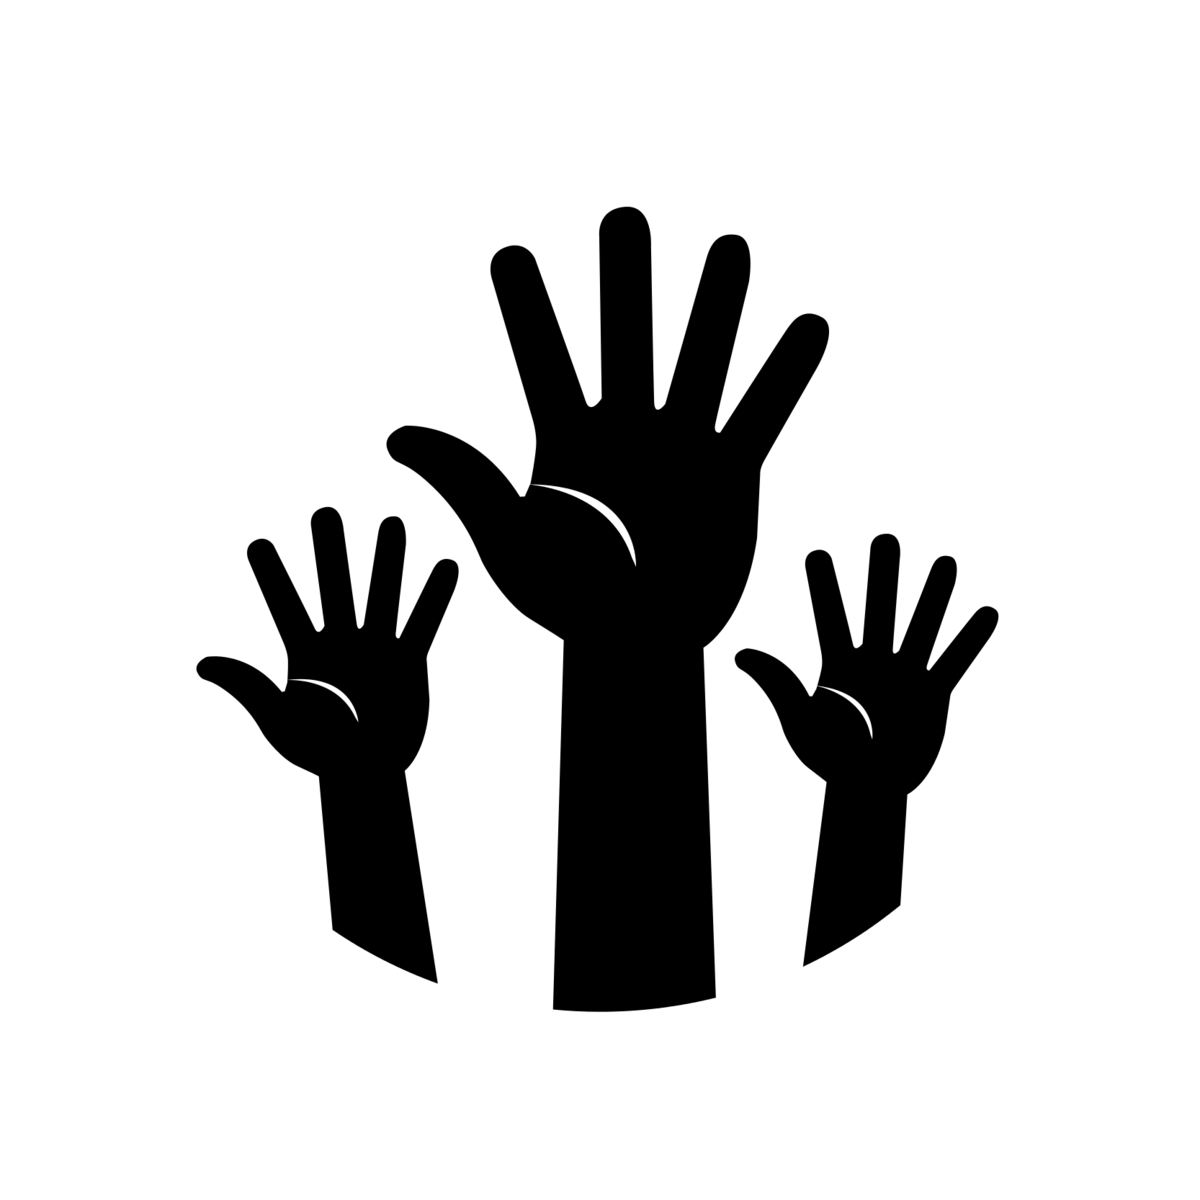
\includegraphics[height=1cm]{images/hands.png}

\end{frame}
%-----------------------------------------------------------------------
%----------------------------------------------------------------------
\begin{frame}[c]{Toy Example: Sequential portfolio}

\begin{itemize}
  \item Runtime cutoff $\kappa = 10$
  \item performance metric $m$: average runtime \onslide<3->{or timeouts}
\end{itemize}

%\medskip

\[
\begin{array}{| r | c  c  c || c | c |}
  \cline{1-6}
      & \algo_1 & \algo_2 & \algo_3 & oracle & Seq. \portfolio\\
  \cline{1-6}
  \inst_1 & 		 1    &         10  &         3    & 1  & 3\\
  \inst_2 &          5    &         10  &  		2 	  & 2 & 6\\
  \inst_3 &          8    &  		1    &         10  & 1 & 3\\
  \inst_4 &         10  &         10  & 		2 	  & 2 & 6\\
  \inst_5 &         10  & 		 6    &         10  & 6 & 10\\
  \inst_6 &         10  &          8    &         10  & 8 & 10\\
  \cline{1-6}
  \onslide<2->{\varnothing & 7.3 & 7.5 & 6.1 & 3.3 & 6.3}\\
  \cline{1-6}
  \onslide<3->{\text{timeouts} & 3 & 3 & 3 & 0 & 2}\\ 
  \cline{1-6}
\end{array}
\]

\onslide<4->{\textit{ppfolio} won many gold medals at the SAT Competition 2011\\ with such a simple approach.}


\end{frame}
%-----------------------------------------------------------------------
%----------------------------------------------------------------------
\begin{frame}[c]{Algorithm Schedules}

\begin{block}{Idea}
Instead of running a uniform schedule with pseudo parallelism (a.k.a. seq. portfolio),
run a non-uniform, ordered schedule of algorithms.
\end{block}

\pause
\begin{itemize}
  \item Runtime cutoff $\kappa = 10$
  \item Schedule: $[\algo_1 \mapsto 1, \algo_3 \mapsto 2, \algo_2 \mapsto 7]$
\end{itemize}

\pause
\[
\begin{array}{| r | c  c  c || c | c c |}
  \cline{1-7}
      & \algo_1 & \algo_2 & \algo_3 & oracle & Seq. \portfolio & Schedule\\
  \cline{1-7}
  \inst_1 & 		 1    &         10  &         3    & 1  & 3 & 1\\
  \inst_2 &          5    &         10  &  		2 	  & 2 & 6 & 3\\
  \inst_3 &          8    &  		1    &         10  & 1 & 3 & 4\\
  \inst_4 &         10  &         10  & 		2 	  & 2 & 6 & 3\\
  \inst_5 &         10  & 		 6    &         10  & 6 & 10 & 9\\
  \inst_6 &         10  &          8    &         10  & 8 & 10 & 10\\
  \cline{1-7}
  \onslide<4->{\varnothing & 7.3 & 7.5 & 6.1 & 3.3 & 6.3 & 5}\\
  \cline{1-7}
  \onslide<5->{\text{timeouts} & 3 & 3 & 3 & 0 & 2 & 1}\\ 
  \cline{1-7}
\end{array}
\]

\end{frame}
%-----------------------------------------------------------------------
%----------------------------------------------------------------------
\begin{frame}[c]{Algorithm Schedules Optimized for Runtime}

\begin{block}{Motivation}
Given a portfolio (set) of algorithms $\portfolio$, a set of instances $\insts$,
runtime as a cost metric and a runtime cutoff $\kappa$
find 
\begin{itemize}
  \item a time slice assignment $\sigma: \portfolio\rightarrow[0,\kappa]$
  \item and a permutation $\rho:\{1,\dots,|\portfolio|\}\rightarrow \portfolio$ 
\end{itemize}
such that the number of timeouts and (average) runtime is minimized.
\end{block}

\pause

\begin{itemize}
  \item Both problems of finding an optimal time slice assignment and a permutation are NP-hard
  \item In practice, too hard to optimize both simultaneously
  \pause 
  \item Two step approach: 
  \begin{enumerate}
    \item find a timeout-minimal time slice assignment $\sigma$
    \item given $\sigma$, find a time-minimal permutation $\rho$
  \end{enumerate}
\end{itemize}
 
\end{frame}
%-----------------------------------------------------------------------
%----------------------------------------------------------------------
\begin{frame}[c]{Time-out minimal Schedule~\litw{Hoos et al. 2015}}

\begin{definition}
Given a portfolio (set) of algorithms $\portfolio$, a set of instances $\insts$,
runtime as a performance metric $t: \portfolio \times \insts \to \perf$,
and a runtime cutoff $\kappa$,
the time-out minimal algorithm scheduling problem 
is to find a schedule $\sigma: \portfolio\rightarrow[0,\kappa]$ such that: 
\[
  \begin{array}{c}
    \sigma
    \in
    \argmax_{\sigma:\portfolio\rightarrow[0,\kappa]}
    |\{\inst \mid t(\algo,\inst)\leq\sigma(\algo), (\algo,\inst)\in{\insts\times \portfolio}\}|
    \\[5pt]
    \text{ such that }\qquad
    \textstyle{\sum}_{\algo \in \portfolio}{\sigma(\algo)} \leq \kappa
  \end{array}
\]
\end{definition}

\medskip
Note: $\sigma$ is an unordered schedule
 
\end{frame}
%-----------------------------------------------------------------------
%----------------------------------------------------------------------
\begin{frame}[c]{Approaches to find a well-performing schedule?}

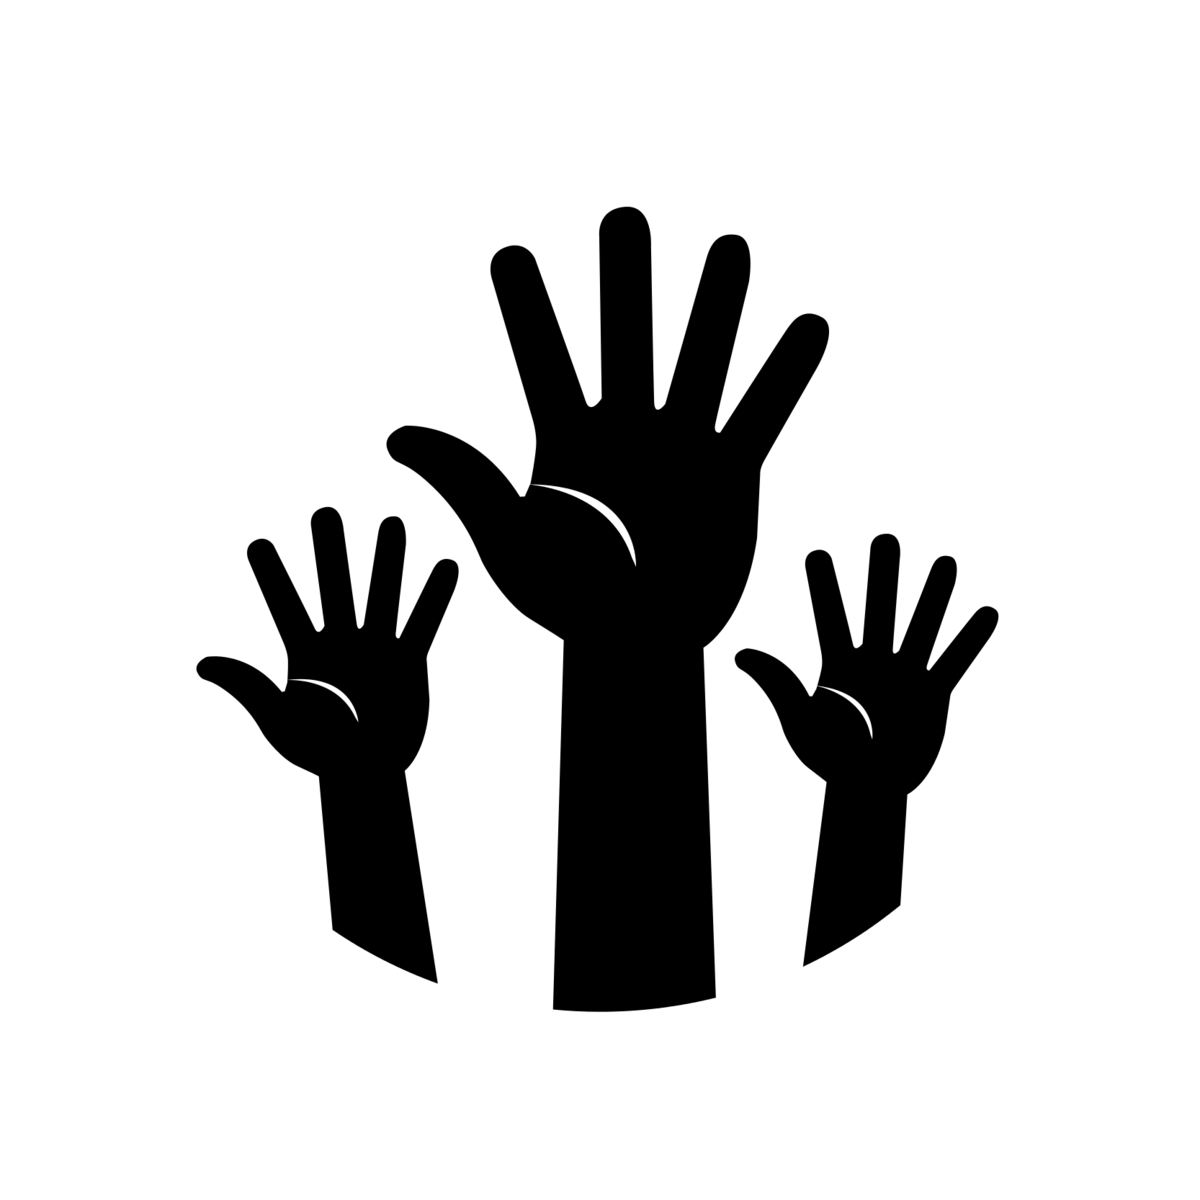
\includegraphics[height=1cm]{images/hands.png}

\bigskip
\pause

\begin{itemize}
  \item Grid search
  \item Random search
  \item Stochastic local search algorithms
  \item Genetic algorithms
  \item Constraint satisfaction problem
  \begin{itemize}
    \item Mixed-Integer Programming
    \item Answer Set Programming
  \end{itemize}
  \item \ldots
\end{itemize}


\end{frame}
%-----------------------------------------------------------------------
%----------------------------------------------------------------------
\begin{frame}[c]{Time-minimal Algorithm Alignment}

\begin{definition}
Given a portfolio (set) of algorithms $\portfolio$, a set of instances $\insts$,
runtime as a cost metric $t: \portfolio \times \insts \to \perf$,
a runtime cutoff $\kappa$,
and an unordered schedule~$\sigma$,
the time-minimal algorithm alignment problem is to find a permutation $\rho$ such that:

	\begin{eqnarray*}
	  \rho
	  & \in & 
	  \argmin_{\rho:\{1,\dots,|\portfolio|\}\rightarrow \portfolio}
	  \textstyle{\sum}_{\inst \in \insts}
	  \tau_{\sigma,\rho}(\inst)\\
%----------------------
	  \tau_{\sigma,\rho}(\inst) & = &
	    \begin{cases} 
	      \left(
	        \textstyle{\sum}_{j=1}^{\min{(P)} - 1}
	        \sigma(\rho(j))
	      \right)
	      +
	      t(\rho(\min{(P)}),\inst)
	       & \text{if $P \not= \emptyset$,}\\
	      \kappa & \text{otherwise}
	    \end{cases}\\
%-----------------------------------
	P & = & \{ l \in \{1,\dots,|\portfolio|\} \mid t(\rho(l),\inst)\leq\sigma(\rho(l)) \}
	\end{eqnarray*}
\end{definition}

\end{frame}
%-----------------------------------------------------------------------
%----------------------------------------------------------------------
\begin{frame}[c,fragile]{Time-minimal Algorithm Alignment: Pseudo-Code}

Pseudo-Python-code to score a permutation $\rho$ given a time slice assignment $\sigma$
and an algorithm portfolio $\portfolio$ of size $k$:

\begin{semiverbatim}
time = 0
for \inst \in \insts:
  for \emph{l} in range(1,k+1):
    if t(\rho(l),\inst) \leq \sigma(\rho(l)):
        time += t(\rho(l),\inst)
        break
    else:
        time += \sigma(\rho(l))
\end{semiverbatim}

\end{frame}
%-----------------------------------------------------------------------
%----------------------------------------------------------------------
\begin{frame}[c]{Algorithm Schedules}

Schedule: $\sigma = \{\algo_1 \mapsto 1, \algo_3 \mapsto 2, \algo_2 \mapsto 7\}$\\
$\rho = \{1 \mapsto \algo_1, 2 \mapsto \algo_3, 3 \mapsto \algo_2\}$


\[
\begin{array}{| r | c  c  c || c | c c |}
  \cline{1-7}
      & \algo_1 & \algo_2 & \algo_3 & oracle & Seq. \portfolio & \sigma\\
  \cline{1-7}
  \inst_1 & 		 1    &         10  &         3    & 1  & 3 & 1\\
  \inst_2 &          5    &         10  &  		2 	  & 2 & 6 & 3\\
  \inst_3 &          8    &  		1    &         10  & 1 & 3 & 4\\
  \inst_4 &         10  &         10  & 		2 	  & 2 & 6 & 3\\
  \inst_5 &         10  & 		 6    &         10  & 6 & 10 & 9\\
  \inst_6 &         10  &          8    &         10  & 8 & 10 & 10\\
  \cline{1-7}
  \varnothing & 7.3 & 7.5 & 6.1 & 3.3 & 6.3 & 5\\
  \cline{1-7}
  \text{timeouts} & 3 & 3 & 3 & 0 & 2 & 1\\ 
  \cline{1-7}
\end{array}
\]

On instance $\inst_2$:\\
$P = \{2\}$\\
\pause
$\tau_{\sigma, \rho} = \sigma(\rho(1)) + t(\inst_2, \rho(2)) = 1 + 2 = 3$

\end{frame}
%-----------------------------------------------------------------------
%----------------------------------------------------------------------
\begin{frame}[c]{Schedules Examples~\litw{Hoos et. al 2015}}

\centering
\begin{tabular}{ l | c  c  c  }
\toprule
   & SAT Crafted & SAT mixed & ASP\\
 \midrule
 Cutoff (sec.) & $5000$ & $5000$ & $900$ \\
 \#Instances  & $300$ & $5467$ & $2432$\\
 \#Algorithms  & $15$ & $37$ & $25$ \\
\bottomrule
\end{tabular}

\bigskip
\pause

\begin{tabular}{ l | r r | r r | r r }
\toprule
 & \multicolumn{2}{c}{SAT Crafted} & \multicolumn{2}{c}{SAT mixed} & \multicolumn{2}{c}{ASP}\\
 \midrule
 Single Best  						& $155$ & $(51.6\%)$ & $1881$ & $(34.4\%)$ & $290$ & $(11.9\%)$\\
 Seq. Schedule       				& $123$ & $(41.0\%)$ & $1001$ & $(18.3\%)$ & $280$ & $(11.5\%)$ \\ 
 \alert{opt. Schedule}				& $98$  & $(32.6\%)$ & $536$ & $(9.8\%)$ & $134$ & $(5.5\%)$\\
 \onslide<3->{\alert{par. Schedule (8)} & $85$  & $(28.3\%)$ & $140$ & $(2.5\%)$ & $56$ & $(2.3\%)$}\\
\bottomrule
\end{tabular}
Number of timeouts (percentage of timeouts)

\end{frame}
%-----------------------------------------------------------------------
%----------------------------------------------------------------------
\begin{frame}[c]{Dynamic Algorithm Portfolios~\litw{Gagliolo and Schmidhuber 2007}}

\begin{block}{Idea}
\begin{itemize}
  \item Collecting training data can be expensive
  \item[$\leadsto$] Try to learn schedule on-the-fly
  \item Adapting time slices over time can be seen as\\ multi-armed bandit problem
\end{itemize}
\end{block}

\pause

\begin{block}{In a nutshell: Multi-Armed Bandit Problem}
\begin{center}
  \includegraphics[width=2.5em]{images/Multi-armed-bandit}
  \includegraphics[width=2.5em]{images/Multi-armed-bandit}
  \includegraphics[width=2.5em]{images/Multi-armed-bandit}
  \includegraphics[width=2.5em]{images/Multi-armed-bandit}
  \includegraphics[width=2.5em]{images/Multi-armed-bandit}
\end{center}
\vspace{-2em}
\begin{itemize}
  \item you are in a casino and have to decide which machine (i.e., arm) to play, how many times and in which order
  \item Each machines provides reward drawn from unknown distribution
  \item Reward distributions are specific to the machine
  \item[$\leadsto$] Trade-off between exploration and exploitation
\end{itemize}
\end{block}

\end{frame}
%-----------------------------------------------------------------------
%----------------------------------------------------------------------
\begin{frame}[c]{Dynamic Algorithm Portfolios~\litw{Gagliolo and Schmidhuber 2007}}

\begin{block}{Idea (cont'd)}
\begin{itemize}
  \item Algorithms are arms in this setting
  \item[$\leadsto$] Play promising arms more often\\ $\approx$ larger time slices for promising algorithms  
\end{itemize}

\pause

\begin{enumerate}
  \item start with a uniform algorithm schedule
  \item for each problem instance $\inst$:
  \begin{enumerate}
    \item run each algorithms $\algo$ with time slice $\sigma(\algo)$ on instance $\inst$
    \item update time slices $\sigma$
    \item if an algorithm solved $\inst$, break
  \end{enumerate}
\end{enumerate}

\pause

Notes: Approach can be improved 
\begin{itemize}
  \item if state of each algorithm is available 
  %\item if intermediate reward signals are available
  \item if similarity between instances is known
\end{itemize}

\end{block}


\end{frame}
%-----------------------------------------------------------------------
%----------------------------------------------------------------------
\begin{frame}[c]{Algorithm Selection~\litw{Rice 1976}}

\begin{block}{Definition}
Given 
\begin{itemize}
  \item a set $\insts$ of problem instances,
  \item a portfolio of algorithms $\portfolio$,
  \item and a cost metric $c:  \portfolio \times \insts \rightarrow \perf$,   
\end{itemize}
 
the \emph{per-instance algorithm selection problem} is to find a mapping 
$s: \insts \rightarrow \portfolio$ 
that optimizes $\sum_{\inst \in \insts} m(s(\inst),\inst)$, 
the sum of performance measures achieved by running the selected algorithm $s(\inst)$ for instance~$\inst$.
\end{block}

\bigskip

\scalebox{0.8}{
\tikzstyle{activity}=[rectangle, draw=black, rounded corners, text centered, text width=8em, fill=white, drop shadow]
\tikzstyle{data}=[rectangle, draw=black, text centered, fill=black!10, text width=8em, drop shadow]
\tikzstyle{myarrow}=[->, thick]
\begin{tikzpicture}[align=center,node distance=3.7cm, thick]
	%PreProcessing
	%\node (PreSolving) [activity, right of=Instance] {Run Pre-Solving Schedule};
	\node (Features) [activity] {Compute\\ Features $\feat(\inst)$};
	\node (Instance) [data, left of=Features] {Instance $\inst$};
	\node (Select) [activity, right of=Features] {Select Algorithm\\ $\feat(\inst) \mapsto \hat{a}$};
	\node (Solve) [activity, right of=Select] {Run $\hat{a}$ on $\inst$};
	\node (Portfolio) [data, above of=Select, yshift=-2.0cm] {Algorithm Portfolio $\portfolio$};

	\draw[myarrow] (Instance) -- (Features);
	%\draw[myarrow] (PreSolving) -- (Features);
	\draw[myarrow] (Features) -- (Select);
	\draw[myarrow] (Select) -- (Solve);
	\draw[myarrow] (Portfolio) -- (Select);
	%\draw[myarrow] (Portfolio) -- (PreSolving);

\end{tikzpicture}
}

\bigskip
\pause
Note: Collecting the training data for the selector can be quite expensive.

\end{frame}
%-----------------------------------------------------------------------
%----------------------------------------------------------------------
\begin{frame}[c]{Instance Features}

\begin{block}{Counting Features}
By analyzing an instance, we can compute some statistics about its characteristics. \\
\end{block}

\bigskip

\begin{block}{Probing Features}
By running an algorithm on an instance for a short amount of time,
we can analyze how the algorithm behaves on this instance.\\
\end{block}

\bigskip
\pause

Please note that there a different names in literature for these types of features.
For example, probing features are related to landmarking features.

\end{frame}
%-----------------------------------------------------------------------
%----------------------------------------------------------------------
\begin{frame}[c]{Instance features: Machine Learning}

\begin{center}
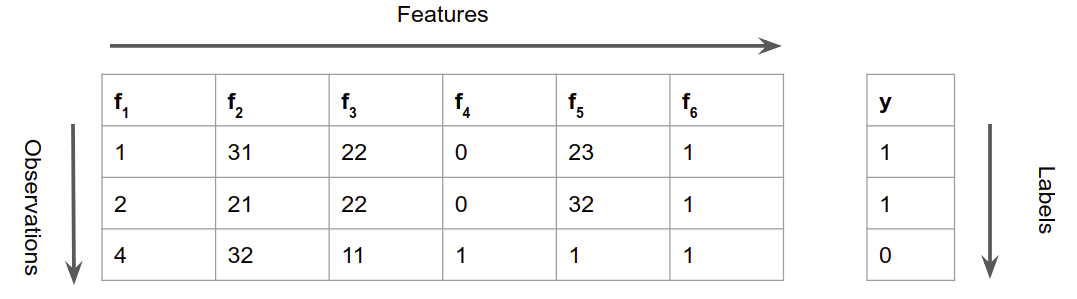
\includegraphics[width=0.9\textwidth]{images/ml_data}
\end{center}


What kind of ``instance features'' could describe a dataset? \hands

\pause
\begin{itemize}
  \item number of observations (samples)
  \item number of features
  \item number of classes
  \item number of categorical features
  \item number of numeric features
  \item percentage of numeric features
  \item number of missing features
  %\item number of observations belonging to most frequent class
  \item Probing: accuracy of a small decision tree
\end{itemize}

\end{frame}
%-----------------------------------------------------------------------
%----------------------------------------------------------------------
\begin{frame}[c]{Instance Features: SAT}

Boolean satisfiability (SAT) instances are encoded as\\ conjunctions of disjunctions of Boolean variables:

$(x_1 \vee x_2)\wedge (x_2 \vee x_3 \vee \neg x_4) \wedge (\neg x_1 \vee x_4) \wedge (\neg x_2 \vee \neg x_3)$

\medskip
\pause
What kind of ``instance features'' could describe such a formula? \hands

\medskip
\pause
\begin{itemize}
  \item number of variables?
  \item number of conjunctions (a.k.a. clauses)
  \item ratio of number of variables and number of clauses
  \pause
  \item Probing feature: number of unsatisfied clauses after running SAT solver for a few seconds 
  \item \ldots
\end{itemize}


\end{frame}
%-----------------------------------------------------------------------
%----------------------------------------------------------------------
\begin{frame}[c]{Instance Features: SAT}

\begin{itemize}
  \item Problem size features (7)
  \item Variable-Clause graph features (10)
  \item Variable graph features (9) (expensive)
  \item Clause graph features (10) (expensive)
  \item Balance features (13)
  \item Proximity to horn formula (7) (expensive)
  \item DPLL Probing Features (7)
  \item LP-based feature (6) (moderate)
  \item Local search probing features (12) (cheap)
  \item Clause learning features (18) (cheap)
  \item Survey propagation feature (18) (moderate)
\end{itemize}

\lit{Algorithm Runtime Prediction: Methods \& Evaluation by Hutter et al. 2014}

\end{frame}
%-----------------------------------------------------------------------
%----------------------------------------------------------------------
\begin{frame}[c]{Instance Features: Runtime~\litw{Xu et al. 2008}}

\centering
\includegraphics[width=1\textwidth]{images/random_indu_feature_rtd.png}

on random instances \hspace{2.2cm}  on industrial instances\

\bigskip
\pause

\flushleft
$\to$ feature computation can be expensive on some instances\\
$\to$ use feature selection to determine an informative but cheap set of features

\end{frame}
%-----------------------------------------------------------------------

%----------------------------------------------------------------------
% \begin{frame}[c]{How to implement an algorithm selector?}
% 
% \begin{center}
% 
\includegraphics[height=1cm]{images/discussion.png}
% \end{center}
% 
% \end{frame}
%-----------------------------------------------------------------------
%----------------------------------------------------------------------
\begin{frame}[c]{\satzilla{}~\litw{Xu et al. 2009}}

\begin{itemize}
  \item one of the prominent approaches for algorithm selection in SAT
  \item won several first places in the SAT competition
  \medskip
  \item Simple idea:
  \begin{enumerate}
    \item use a static algorithm schedule (called pre-solving schedule)
    \item if the pre-solving schedule failed to solve the instance at hand,\\
    		compute the instance features of the instance
    \item run the algorithm with the best predicted performance
    	  \begin{itemize}
    	    \item use a regression model to predict the performance of each algorithm\\
    	    ($\to$ $k$ regression models for $k$ algorithms in the portfolio)
    	  \end{itemize}
  \end{enumerate}
\end{itemize}

\end{frame}
%-----------------------------------------------------------------------
%----------------------------------------------------------------------
\begin{frame}[c]{Literature}

\begin{itemize}
  \item \lit{SATzilla: Portfolio-based Algorithm Selection for SAT. L. Xu, F. Hutter, H. H. Hoos, K. Leyton-Brown - Journal of Artificial Intelligence Research, Volume 32, pp. 565–606, 2008}
  \item \lit{Lars Kotthoff. Algorithm Selection for Combinatorial Search Problems: A Survey. AI Magazine, 2014}
  \item Literature overview: \url{http://larskotthoff.github.io/assurvey/}
\end{itemize}


\end{frame}
%-----------------------------------------------------------------------
%----------------------------------------------------------------------
\begin{frame}[c]{Learning Goals}

After this lecture, you will be able to \ldots

\begin{itemize}
  \item \alert{exploit complementarity} of algorithms to improve overall performance
  \item explain \alert{algorithm portfolios} and its different variants
  \begin{itemize}
    \item racing portfolios
    \item parallel portfolios
    \item algorithm schedules
  \end{itemize}
  \item define \alert{per-instance algorithm selection} and to describe one specific implementation 
  \item explain different types of \alert{instance features}
\end{itemize}

\end{frame}
%-----------------------------------------------------------------------